\documentclass[twoside,leqno,twocolumn]{article}
\usepackage{ltexpprt}

%\documentstyle[nips07submit_09,times]{article}

\usepackage{amsmath,amssymb}
\usepackage{graphicx}

% Standardized pseudocode functions
\newcommand{\spos}{^{{\scriptscriptstyle +\!}}}
\newcommand{\sneg}{^{{\scriptscriptstyle -\!}}}

\DeclareMathOperator*{\map}{map}
\DeclareMathOperator*{\argmin}{argmin}
\DeclareMathOperator*{\argmax}{argmax}

\DeclareMathOperator{\enqueue}{enqueue}
\DeclareMathOperator{\dequeue}{dequeue}

\DeclareMathOperator{\tpc}{tpc}
\DeclareMathOperator{\rng}{rng}
\DeclareMathOperator{\allnn}{allnn}
\DeclareMathOperator{\kde}{kde}
\DeclareMathOperator{\kda}{kda}
\DeclareMathOperator{\contrib}{\delta}

\newcommand{\peq}{\mathrel{\mathord{+}\mathord{=}}}
\newcommand{\meq}{\mathrel{\mathord{-}\mathord{=}}}
\newcommand{\maxeq}{\mathbin{\mathord{\max}\mathord{=}}}
\newcommand{\mineq}{\mathbin{\mathord{\min}\mathord{=}}}
\newcommand{\comp}{\mathbin{\circ}}

\newcommand{\GenOp}[1]{\mathop{\bigotimes\nolimits_{\lefteqn{\scriptstyle \!#1}}}}
\newcommand{\genop}[1]{\mathbin{\otimes_{\scriptscriptstyle \!#1}}}

\newcommand{\Gnp}{\Psi}
\newcommand{\gnp}{\psi}

\newcommand{\XX}{~~}
\newcommand{\X}{\\} %\scriptstyle
\newcommand{\x}{\X \XX}
\newcommand{\xx}{\X \XX\XX}
\newcommand{\xxx}{\X \XX\XX\XX}
\newcommand{\xxxx}{\X \XX\XX\XX\XX}
\newcommand{\xlet}{{\bf let}\:}
\newcommand{\xif}{{\bf if}\:}
\newcommand{\xelif}{{\bf elif}\:}
\newcommand{\xelse}{{\bf else}\:}
\newcommand{\xwhile}{{\bf while}\:}
\newcommand{\xreturn}{{\bf return}\:}
\newcommand{\xfunction}{{\bf function}\:}
\newcommand{\xinit}{{\bf init}\:}

\newcommand{\kdroot}[1]{#1^{\rm root}}
\newcommand{\kdleft}[1]{#1^{\!L}}
\newcommand{\kdright}[1]{#1^{\!R}}
\newcommand{\kdparent}[1]{#1^{\!P}}

\newcommand{\lo}[1]{#1^{l}}
\newcommand{\hi}[1]{#1^{u}}
\newcommand{\lohi}[1]{#1^{l,u}}
\newcommand{\hilo}[1]{#1^{u,l}}



\title{Towards a Calculus of Massive-Scale Machine Learning}
\author{Ryan N.~Riegel --
    Georgia Institute of Technology --
    \texttt{rriegel@cc.gatech.edu}
}
\date{}

\begin{document}

\maketitle

\section{Introduction}
Machine Learning (ML) methods have recently seen a wide range of
applications in statistics, the natural sciences, engineering, and
Internet services.  Obvious implementations of many such methods are
$O(N^2)$ or worse, rendering them infeasible on large data sets, but a
new algorithmic strategy \cite{nips2000paper} inspired by
breakthroughs in computational physics \cite{appel2, barnes_hut,
grngard} provides hope for a wide range of computations dubbed {\em
Generalized $N$-body Problems} (GNPs).  This algorithmic strategy has
been applied to a succession of well-known statistical learning
methods, including the all-$k$-nearest-neighbors problem
\cite{nips2000paper}, kernel density estimation \cite{nips2000paper,
kde-siamdm, kde-nips-dong, kde-uai-dong}, $k$-nearest-neighbor
classification \cite{ting-liu}, kernel discriminant analysis (KDA)
\cite{nbc-compstat}, and the $n$-point correlation
\cite{nips2000paper, moore-npt}.  Further, these algorithms have been
demonstrated on large scientific datasets, producing first-of-a-kind
high-profile results \cite{science03, nature05}.  For each of these
problems, no overall faster algorithms are known.  In addition, these
algorithms compute either exact results or approximations to within
specified bounds on absolute or relative error, a rarity amongst fast
methods.

In this proposal, we wish to show that the Microsoft Research
Fellowship would help us redefine the state of the art in
computational methods, potentially changing the face of science.  We
begin with several examples of our work followed by a brief look at
the underlying mathematics.  We then explain our most recent
applications and finish with a description of the road ahead.

\section{Examples}
GNPs typically make use of spatially-informed trees, such as the
$kd$-trees \cite{preparata} shown in Figure~\ref{fig:kd-trees}.  These
do not in general have to be binary or balanced, but for the purpose
of these examples, we assume that they are.  Symbols $X$, $Q$, and $R$
denote tree nodes and their represented data; $\kdleft{X}$ and
$\kdright{X}$ are the nodes' children and $\kdroot{X}$ is the entire
data set.  Another concept present in all GNPs is that of bounded
intermediate results, often derived from distance bounds.  For metric
$d$ and sets $X_1$ and $X_2$, upper and lower bounds $\hi{d}(X_1,X_2)$
and $\lo{d}(X_1,X_2)$ are obtained from, for instance, bounding boxes
formed on the data.  All GNPs work by tightening bounds in a
high-order divide-and-conquer manner until conclusions can be made
about the final result.

\begin{figure}[tb]
  \begin{center}
    \begin{minipage}{1.05in}
      \includegraphics[width=1.0in]{kdtree-level2.ps}
    \end{minipage}
    \begin{minipage}{1.05in}
      \includegraphics[width=1.0in]{kdtree-level4.ps}
    \end{minipage}
    \begin{minipage}{1.05in}
      \caption{\label{fig:kd-trees}\footnotesize Depths 2 (left) and 4
	(right) of a 2D $kd$-tree.}
    \end{minipage}
  \end{center}
  \vspace{-10pt}
\end{figure}

\subsection{The $n$-point Correlation.}
The $n$-point correlation measures fractal dimension by computing the
number of groups of $n$ points all within some radius $h$ of each
other.  In the case that $n = 2$, this is given by\footnote{Simple
methods may prevent the recounting of permutations.}
\begin{equation}
  \sum_{x_1 \in X} \sum_{x_2 \in X} I(d(x_1,x_2) \leq h) ,
\end{equation}
where $I$ is the indicator function.  This is obviously quadratic when
implemented as a nested loop, but the dual-tree\footnote{Multi-tree
algorithms are also possible for $n > 2$.} equivalent in
Figure~\ref{fig:tpc} is empirically $O(N^{1+\epsilon})$
\cite{nips2000paper}.  This algorithm achieves its acceleration by
{\em pruning} work on paired nodes when bounding boxes prove them to
be entirely outside or within radius $h$ of each other.

\begin{figure}[tb]
  \begin{center}\fbox{\begin{minipage}{3.1in}
  \begin{displaymath}
    \begin{array}{l}
      \xfunction \tpc(X_1,X_2)
      \x \xif \lo{d}(X_1,X_2) > h,\:\xreturn 0
      \x \xif \hi{d}(X_1,X_2) \leq h,\:\xreturn |X_1| \cdot |X_2|
      \x \xreturn \tpc(\kdleft{X_1},\kdleft{X_2}) + \tpc(\kdleft{X_1},\kdright{X_2})
      \xx \mbox{} + \tpc(\kdright{X_1},\kdleft{X_2}) + \tpc(\kdright{X_1},\kdright{X_2})
    \end{array}
  \end{displaymath}
  \end{minipage}}\end{center}
  \vspace{-10pt}
  \caption{\label{fig:tpc}\footnotesize Dual-tree two-point correlation.}
\end{figure}

\subsection{Range Count.}
A minor modification of the two-point correlation reports separate
sums for each point rather than adding them all together.  For queries
$Q$ and references $R$, this range count problem is given by
\begin{equation}
  \map_{q \in Q} \sum_{r \in R} I(d(q,r) < h) ,
\end{equation}
where $\map_{x \in X} f(x) = \{(x, f(x)) | x \in X\}$ returns a set of
key-value pairs.  The algorithm in Figure~\ref{fig:rng} maintains a
vector of results $a$, but prunes the same as before.

\begin{figure}[tb]
  \begin{center}\fbox{\begin{minipage}{3.1in}
  \begin{displaymath}
    \begin{array}{l}
      \xinit \forall q \in \kdroot{Q}, a(q) = 0 \\
      \xfunction \rng(Q,R)
      \x \xif \hi{d}(Q,R) \leq h,\:\forall q \in Q, a(q) \peq |R|
      \x \xelif \lo{d}(Q,R) \leq h,
      \xx \rng(\kdleft{Q},\kdleft{R});\:\rng(\kdleft{Q},\kdright{R})
      \xx \rng(\kdright{Q},\kdleft{R});\:\rng(\kdright{Q},\kdright{R})
    \end{array}
  \end{displaymath}
  \end{minipage}}\end{center}
  \vspace{-10pt}
  \caption{\label{fig:rng}\footnotesize Dual-tree range count.}
\end{figure}

\subsection{All-nearest-neighbors.}
In applications ranging from classification to manifold learning, it
is useful to find nearest neighbors to each of a set of query points,
\begin{equation}
  \map_{q \in Q} \argmin_{r \in R} d(q,r) .
\end{equation}
As shown in Figure~\ref{fig:allnn}, pruning occurs when the
lower-bound distance from $Q$ to $R$ is greater than all of $Q$'s
candidate nearest neighbor distances.  Unlike the above, pruning
depends on previous work; in practice, depth-first traversal visiting
nearer nodes first is fastest.

\begin{figure}[tb]
  \begin{center}\fbox{\begin{minipage}{3.1in}\vspace{-10pt}
  \begin{displaymath}
    \begin{array}{l}
      \xinit \forall q \in \kdroot{Q}, a(q) = \infty \\
      \xfunction \allnn(Q,R)
      \x \xif \hi{a}(Q) \leq \lo{d}(Q,R),\:\xreturn
      \x \xif (Q,R)=(\{q\},\{r\}),
      \xx a(q) = \min\{a(q),d(q,r)\};\:\xreturn
      \x \text{prioritize } \{R^1,R^2\} = \{\kdleft{R},\kdright{R}\} \text{ by } \lo{d}(\kdleft{Q},\cdot)
      \xx \allnn(\kdleft{Q},R^1);\:\allnn(\kdleft{Q},R^2)
      \x \text{prioritize } \{R^1,R^2\} = \{\kdleft{R},\kdright{R}\} \text{ by } \lo{d}(\kdright{Q},\cdot)
      \xx \allnn(\kdright{Q},R^1);\:\allnn(\kdright{Q},R^2)
    \end{array}
  \end{displaymath}
  \end{minipage}}\end{center}
  \vspace{-10pt}
  \caption{\label{fig:allnn}\footnotesize Dual-tree all-nearest-neighbors.}
\end{figure}

\subsection{Kernel Density Estimation.}
Probability distributions that are hard to model may nonetheless
be accurately estimated from data via a kernel summation,
\begin{equation}
  \map_{q \in Q} \frac{1}{|R|} \sum_{r \in R} K_h(q,r) ,
\end{equation}
where $K_h$ may be the Gaussian or Epanechnikov kernels, among others.
To accelerate general kernel summations, we can use approximation with
bounded error, a rudimentary form of which is shown in
Figure~\ref{fig:kde}.  More advanced methods are described in
\cite{kde-nips-dong, kde-uai-dong}.

\begin{figure}[tb]
  \begin{center}\fbox{\begin{minipage}{3.1in}\vspace{-10pt}
  \begin{displaymath}
    \begin{array}{l}
      \xinit \forall q \in \kdroot{Q}, a(q) = 0;\:b = 0 \\
      \xfunction \kde(Q,R,b)
      \x \xif \hi{K_h}(Q,R) - \lo{K_h}(Q,R) < (\lo{a}(Q)+b)\frac{|R| \cdot \epsilon}{|\kdroot{R}|},
      \xx \forall q \in Q, a(q) \peq \lo{K_h}(Q,R);\:\xreturn
      \x \text{prioritize } \{R^1,R^2\} = \{\kdleft{R},\kdright{R}\} \text{ by } \lo{d}(\kdleft{Q},\cdot)
      \xx \kde(\kdleft{Q},R^1,b+\lo{K_h}(\kdleft{Q},R^2));\:\kde(\kdleft{Q},R^2,b)
      \x \text{prioritize } \{R^1,R^2\} = \{\kdleft{R},\kdright{R}\} \text{ by } \lo{d}(\kdright{Q},\cdot)
      \xx \kde(\kdright{Q},R^1,b+\lo{K_h}(\kdright{Q},R^2));\:\kde(\kdright{Q},R^2,b)
    \end{array}
  \end{displaymath}
  \end{minipage}}\end{center}
  \vspace{-10pt}
  \caption{\label{fig:kde}\footnotesize Dual-tree kernel density estimation.}
\end{figure}

\subsection{Kernel Discriminant Analysis.}
The Bayes' optimal classifier on two classes assigns observation $q$
to the class $C$ with the greatest posterior probability $P(C|x)
\propto f(x|C)P(C)$, where $f(x|C)$ may be estimated with the above.
We formulate this KDA with
\begin{equation}
  \map_{q \in Q} \argmax_{C \in \{C_1,C_2\}} \frac{P(C)}{|R_C|} \sum_{r \in R_C} K_{h_C}(q,r) ,
\end{equation}
where $R_C$ is the subset of references from $C$ and $h_C$ is a
class-dependent bandwidth.  A fast algorithm for this problem
\cite{nbc-compstat} maintains bounds on $f(x|C_1)$ and $f(x|C_2)$,
terminating on sets of queries when one class' lower-bound probability
exceeds the other's upper-bound.  Recent efforts have made further
improvements to running time, such as the breadth-first work order in
Figure~\ref{fig:kda}.

\begin{figure}[tb]
  \begin{center}\fbox{\begin{minipage}{3.1in}\vspace{-10pt}
  \begin{displaymath}
    \begin{array}{l}
      \xinit \forall q \in \kdroot{Q}, a(q) = \contrib(\kdroot{Q},\kdroot{R}) \\
      \enqueue(\kdroot{Q},\kdroot{R}) \\
      \xwhile \dequeue(Q,R) \quad \text{// Main loop of } \kda
      \x \xif \lo{a}(Q) > 0 \text{ or } \hi{a}(Q) < 0, \xreturn
      \x \forall q \in Q, a(q) \meq \contrib(Q,R)
      \x \forall q \in \kdleft{Q}, a(q) \peq \contrib(\kdleft{Q},\kdleft{R}) + \contrib(\kdleft{Q},\kdright{R})
      \x \forall q \in \kdright{Q}, a(q) \peq \contrib(\kdright{Q},\kdleft{R}) + \contrib(\kdright{Q},\kdright{R})
      \x \enqueue(\kdleft{Q},\kdleft{R});\:\enqueue(\kdleft{Q},\kdright{R})
      \x \enqueue(\kdright{Q},\kdleft{R});\:\enqueue(\kdright{Q},\kdright{R})
      \\ \\
      \xfunction \contrib(Q,R)
      \x \xreturn |R_{C_1}| \cdot \lohi{K_{h_{C_1}}}(Q,R_{C_1}) P(C_1)
      \xx \mbox{} - |R_{C_2}| \cdot \hilo{K_{h_{C_2}}}(Q,R_{C_2}) P(C_2)
    \end{array}
  \end{displaymath}
  \end{minipage}}\end{center}
  \vspace{-10pt}
  \caption{\label{fig:kda}\footnotesize Dual-tree kernel discriminant analysis.}
\end{figure}

\section{Generalized $N$-body Problems}
As is apparent from the examples, problems that benefit from
multi-tree algorithms have a very characteristic form.  GNPs are
high-order reductions $\Gnp = g \comp \gnp$, with
\begin{equation}
  \gnp(X_1,\ldots,X_n) = \GenOp{1}_{x_1 \in X_1} \cdots \GenOp{n}_{x_n \in X_n} f(x_1,\ldots,x_n)
\end{equation}
subject to decomposability requirement, for $1 \leq i \leq n$,
\begin{equation}
  \gnp(\ldots,X_i,\ldots) = \gnp(\ldots,\kdleft{X_i},\ldots) \genop{i} \gnp(\ldots,\kdright{X_i},\ldots) .
\end{equation}
That is, there is an inner function $f$, a series of commutative,
associative operators $\genop{i}$ performing reductions over the input
data, and possibly an outer function $g$ to finalize results; further,
the order of computation must be fairly flexible.  Decomposability is
always possible when the operators $\genop{i}$ form a combination of
$\map$ and some one other operator.  Some other situations permit
decomposition, but even when it is not immediately possible,
transformations may be employed to render problems into GNPs or nested
GNPs.  For instance, an outer operator may be replaced with $\map$,
thereby collecting a set of results to be processed afterward.

Despite the diversity of GNPs, there exists one algorithm to solve
them all, given by $\gnp(X_1,\ldots,X_n) =$
\begin{equation}
  \left\{ \!\!\! \begin{array}{lrrr}
    a & \multicolumn{3}{r}{\text{if bounds prove it is safe to prune to $a$},} \\
    \multicolumn{2}{l}{f(x_1,\ldots,x_n)} & \multicolumn{2}{r}{\text{if } X_i = \{x_i\}, 1 \leq i \leq n,} \\
    \multicolumn{3}{l}{\gnp(\ldots,\kdleft{X_i},\ldots) \genop{i} \gnp(\ldots,\kdright{X_i},\ldots)} & \text{otherwise},
  \end{array} \!\!\! \right.
\end{equation}
where split set $X_i$ is selected based on, say,
size\footnote{Alternately, all sets may be split simultaneously.} and
partitions $\kdleft{X_i}$ and $\kdright{X_i}$ are decided quickly, as
by a tree.  Pruning may take several forms.  For instance, as in the
$n$-point correlation, it may depend solely upon bounds on local
computation $\psi(X_1,\ldots,X_n)$.  Alternately, as in
all-nearest-neighbors, pruning may involve comparing bounds on past
work and bounds on $\psi(X_1,\ldots,X_n)$.  Or, as in KDA, pruning may
depend only on bounds on past work.  Each of these has different
implications regarding how work should progress (e.g.~depth-first
vs.~breadth-first).

\section{GNPs in Recent ML: Affinity Propagation}
To demonstrate the versatility of the above, we apply it to affinity
propagation \cite{affinity}, a recent clustering technique that
identifies cluster exemplars within a data set.  For similarity matrix
$S$ with parameters influencing the number of exemplars along its
diagonal, the standard algorithm alternatingly updates matrices $R$
and $A$ with
\begin{align}
  r_{ij} & \gets s_{ij} - \max_{j' \neq j} (a_{ij'} + s_{ij'}) , \\
  a_{ij} & \gets \kappa^-_{ij} \Big( \sum_{i' \neq i} \kappa^+_{i'j}(r_{i'j}) \Big) ,
\end{align}
where $\kappa^{\pm}_{ij}(v)$ clamps $v$ to be positive or negative if
$i \neq j$ and returns $v$ unmodified otherwise.  To prevent
oscillations, it helps to damp the values of $R$ and $A$ with $R \gets
(1 - \lambda) R^{\rm new} + \lambda R^{\rm old}$, etc.  Exemplars are
then the points $k$ maximizing $a(i,k) + r(i,k)$ for the various $i$.

In order to scale to very large data sets, the normal algorithm
permits $S$ to be sparse, but this introduces an uncontrolled amount
of error.  Alternately, if $\lambda = 0$ and similarity is a function
of metric distance, we may pose affinity propagation as vectors
$\alpha$ and $\rho$, defined
\begin{align}
  \alpha_i & \gets \mathop{\argmin\nolimits^2}_j (\kappa^+_{ij}(\kappa^+_{ij}(s_{ij} + \alpha_{i[j]}) - \rho_j) - s_{ij}) , \\
  \rho_j & \gets \sum_i \kappa^+_{ij}(s_{ij} + \alpha_{i[j]}) ,
\end{align}
where $\argmin\nolimits^2$ finds the two smallest values and
$\alpha_{i[j]}$ returns the smallest value if its index is not $j$ and
the second smallest value otherwise.  Exemplars can be shown to be the
points $k$ for which $\rho_k$ is positive.

These computations constitute GNPs and may be solved efficiently with
algorithms similar to those of all-nearest-neighbors and kernel
density estimation.  The only drawback is the absence of standard
damping; oscillations must be discouraged by other means.  Our overall
space requirement is $O(N)$ and our per-iteration running time, shown
in Figure~\ref{fig:ap-speed}, is empirically $O(N^{1.3})$ on 3D data.
This translates to dramatic improvements in scalability: full matrices
$R$ and $A$ would be multiple terabytes for one million points, but
our algorithm can perform an iteration at that size in about 100
seconds, an extrapolated 300 times faster than standard.

\begin{figure}[tb]
  \begin{center}
    \includegraphics[width=0.45\textwidth]{r-speed.ps}
  \end{center}
  \vspace{-10pt}
  \caption{\label{fig:ap-speed}\footnotesize Mean per-iteration
    running times for affinity propagation.  The Frey-Dueck curve is
    extrapolated after running out of memory at 10k points.
    Parameter $p$ is the median similarity, itself found via a GNP.
    Code compiled by gcc 3.4.6 in Linux 2.6.9 on a NetBurst-class
    Intel Xeon 3.0GHz with 8GB RAM.}
\end{figure}

\section{GNPs in the Sciences: Quasar Identification}
Quasars are star-like objects that are not very well understood, yet
play a critical role in cosmology.  As the most luminous objects in
the universe, they may be used as markers of mass in the very
distant/early universe, making them invaluable to the verification of
theories such as dark energy.  Prior to our work, the largest
available catalog of quasars listed fewer than one hundred thousand
examples; massive sky surveys such as the Sloan Digital Sky Survey
(SDSS), on the other hand, are expected to contain millions.  The
challenge is then to identify quasars given the information made
available by the survey: brightness and color spectra.

In \cite{richards04} and continuing work with our physicist
collaborators, we trained a KDA classifier using 4D spectra data from
a relatively small set (80k) of known quasars and many (400k)
non-quasars.  We have so far identified approximately one million
quasars from the SDSS data (40m); further, hand-verification of a
subset of our results suggests that they are highly accurate.  Using
bandwidths estimated from training data by a work-sharing
multi-bandwidth version of the algorithm, the entire classification
takes approximately 30 minutes on a single computer.  Already, an
earlier rendition of our catalog has been used to confirm the cosmic
magnification effect predicted by relativity \cite{nature05}.

\section{How the MSR Fellowship Would Help}
In an ongoing Microsoft seed effort, ``Data Mining Everywhere,'' we
are porting the above methods to Microsoft products such as SQL Server
and Excel.  This, however, will barely touch upon the full scope of
generalized $N$-body problems.  Already in our sights are additional
data mining techniques such as GP regression, manifold learning, and
PCA.  If awarded, the very least that the Microsoft Research
Fellowship would enable is the development of fast algorithms for
dozens of other computational problems, all of which would become
available to any user of Microsoft products.

In another line of work, we strive to extend our algorithmic
technique's already high scalability to handle ultra-massive data sets
such as the Internet and cutting-edge scientific experiments, some of
which produce gigabytes of data per second.  We have already
implemented a framework that automatically parallelizes a limited
selection of GNPs over multiple cores and/or machines.  Further
generalization of this framework and porting it to Microsoft products
would allow users to make the most of their computational resources.
In addition, the Microsoft Research Fellowship would allow us to
pursue what is effectively the final frontier of scalability: Monte
Carlo methods, or a controlled form of subsampling that offers
probabilistic error bounds.  We conjecture that Monte Carlo methods
may be applied generally to all GNPs, thereby allowing magnified
scalability at the flick of a switch.

The true Holy Grail of our efforts, however, is to enable end-users
(not necessarily end-{\em programmers}) to specify custom
computational problems, such as we could never anticipate, and still
benefit from the scalability inherent in GNPs.  The parallelization
framework already in existence only requires the fill-in of a handful
of function stubs, but these may be derived from the operators that
define the GNP.  We envision a system in which the user needs only
work in terms of mathematical symbols, with a code-generator compiling
these into an efficient, massively scalable algorithm, ideally in the
user's language of choice.  We will break ground on this ambitious
project in a matter of weeks, but ultimately we will need more funding
to see our goals to fruition.  Securing the Microsoft Research
Fellowship would be of great assistance in the nascent stages of this
work.

{\footnotesize
\bibliographystyle{abbrv}
\bibliography{ms_prop}
}

\end{document}
